\documentclass{training}
\setlang{french}
% Filigrane PAR MODULE : \uxfond (PNG A4 dilue 30 %). Cadre noir vectoriel commun.
% Proportions original 744 px : marge 20/744, trait 1/744. Exterieur BLANC.
% Cadre via eso-pic +\put (coordonnees absolues) — pas de remember picture (decalage).
\usepackage{eso-pic}

\providecommand{\uxfond}{../../resources/fond/norme_fond_paliers_30.png}

\newlength{\uxmargin}
\newlength{\uxthick}
\newlength{\uxinnerw}
\newlength{\uxinnerh}
\setlength{\uxmargin}{0.02688\paperwidth}% 20/744
\setlength{\uxthick}{0.001344\paperwidth}% 1/744
\setlength{\uxinnerw}{\dimexpr\paperwidth-2\uxmargin-2\uxthick\relax}
\setlength{\uxinnerh}{\dimexpr\paperheight-2\uxmargin-2\uxthick\relax}

% Contenu strictement a l'interieur du trait (+ jour confortable).
\geometry{%
  includeheadfoot,
  left=22mm,
  right=22mm,
  top=20mm,
  bottom=18mm,
  headheight=30pt,
  headsep=5mm,
  footskip=12mm%
}

\AddToShipoutPictureBG{%
  \AtPageLowerLeft{%
    % Fond blanc page entiere
    \put(0,0){\color{white}\rule{\paperwidth}{\paperheight}}%
    % Filigrane module a l'interieur du cadre
    \put(\LenToUnit{\dimexpr\uxmargin+\uxthick\relax},\LenToUnit{\dimexpr\uxmargin+\uxthick\relax}){%
      \includegraphics[width=\uxinnerw,height=\uxinnerh]{\uxfond}}%
    % Cadre noir : bas, haut, gauche, droite
    \put(\LenToUnit{\uxmargin},\LenToUnit{\uxmargin}){%
      \color{black}\rule{\dimexpr\paperwidth-2\uxmargin\relax}{\uxthick}}%
    \put(\LenToUnit{\uxmargin},\LenToUnit{\dimexpr\paperheight-\uxmargin-\uxthick\relax}){%
      \color{black}\rule{\dimexpr\paperwidth-2\uxmargin\relax}{\uxthick}}%
    \put(\LenToUnit{\uxmargin},\LenToUnit{\uxmargin}){%
      \color{black}\rule{\uxthick}{\dimexpr\paperheight-2\uxmargin\relax}}%
    \put(\LenToUnit{\dimexpr\paperwidth-\uxmargin-\uxthick\relax},\LenToUnit{\uxmargin}){%
      \color{black}\rule{\uxthick}{\dimexpr\paperheight-2\uxmargin\relax}}%
  }%
}

\makeatletter
\fancyhf{}
\fancyheadoffset{0pt}
\renewcommand{\headrulewidth}{0pt}
\lhead{\parbox[t]{0.56\textwidth}{\RaggedRight\footnotesize\sloppy\@title}}
\rhead{\parbox[t]{0.36\textwidth}{\RaggedLeft\footnotesize\sloppy\@subtitle}}
\cfoot{\thepage}
% Coupures : underscore et slash dans les noms de fichiers / consignes
\DeclareRobustCommand{\_}{\textunderscore\allowbreak}
\makeatother

% Evite les depassements de longues lignes (Github, Name_FirstName_...)
\sloppy
\emergencystretch=3em
\hbadness=10000

% Sommaire type 42 : chapitres seulement
\setcounter{tocdepth}{0}
\renewcommand{\cftchappresnum}{}
\renewcommand{\cftchapaftersnum}{}
\setlength{\cftchapnumwidth}{2.0em}
\setlength{\cftbeforechapskip}{0.35em}
\cftsetindents{chapter}{0em}{2.0em}


\begin{document}

\schoollogo{../../resources/jeunecrack.png}
\title{Athlète, hydrate-toi}
\subtitle{Piscine UX/UI --- UX}
\member{Piscine UX/UI}{https://github.com/01-edu/UX-UI}
\summary{Une réponse non numérique à la façon dont les coureurs boivent.}
\version{1.0}
\prerequisite{Le module précédent de cette piscine, ou aucun si c'est le premier.}
\maketitle

\newpage
\tableofcontents
\newpage


\chapter{Instructions}

L'avant-propos n'est pas un exercice. Il ne sera pas noté. Les exercices commencent au chapitre suivant, du contrat le plus simple au plus dur. Un exercice plus tardif n'est pas pris en compte si un plus tôt ne tient pas.

On ne regarde que ce qui est dans le répertoire de rendu de l'exercice. N'ajoutez pas un fichier que l'exercice ne nomme pas. Le nom d'un livrable suit le motif imprimé dans l'exercice : \texttt{Name\_FirstName\_DeliverableName\_Date\_VersionNumber}.

Le geste ne vous est pas donné. Les exemples d'un exercice portent parfois une contrainte que la phrase ne répète pas. Lisez-les. Vos autres références sont le manuel de l'outil choisi, la personne assise à côté, et les liens imprimés dans l'exercice.

L'ordre est celui de la quête. Sauter une étape parce qu'un écran plus tard semble plus intéressant produit un écran que personne ne sait expliquer.

\subsection*{Des images}

La marque en couverture est le logo du projet. L'image de l'avant-propos est l'illustration de ce module. Le fond pâle derrière le texte est le filigrane de page. Aucun n'est un indice.

\subsection*{Des machines qui écrivent}

Vous pouvez vous servir d'un outil pour vérifier un mot, comme d'un dictionnaire. Vous ne pouvez pas remplacer un entretien, un test ou un fichier par un texte généré et le signer. Si vous ne pouvez pas montrer la personne, l'écran ou la ligne que vous avancez, l'exercice n'est pas fait.


\chapter{Avant-propos}

Avant les écrans, il y a la route. \emph{Les Chariots de feu} (Hugh Hudson, 1981) suit deux coureurs et ne s'attarde pas sur l'objet qui les sauvera. Cette quête est de cet acabit : le problème d'hydratation est réel, et le rendu n'a pas à être une application. Le film ne dit pas quoi fabriquer. Cette page non plus.

\begin{center}
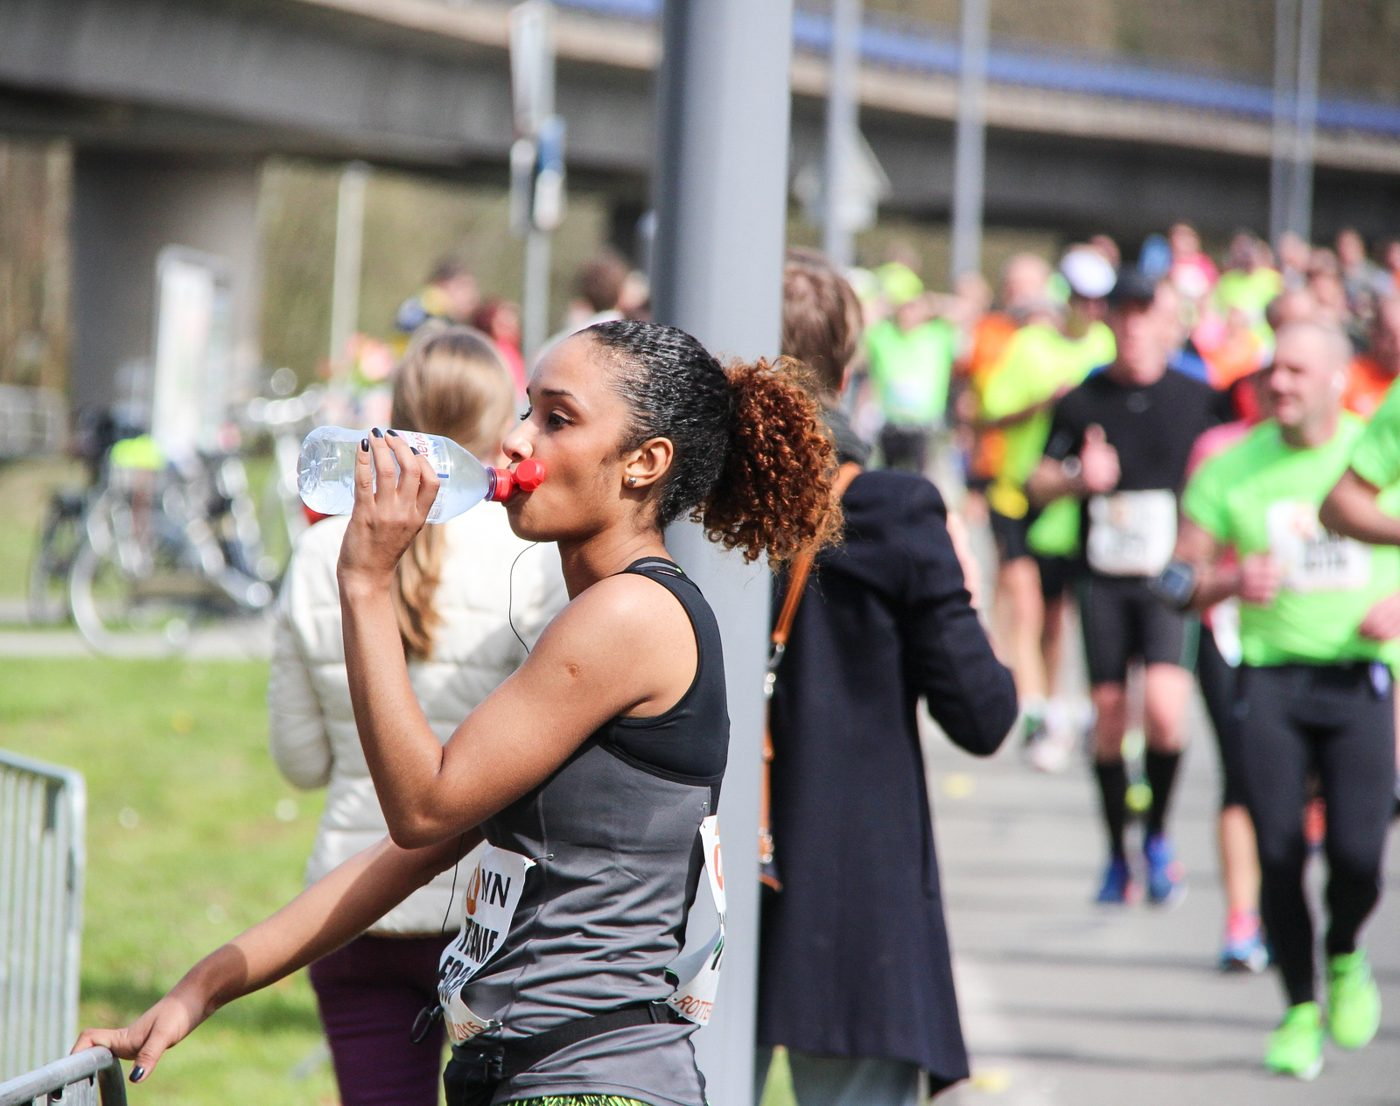
\includegraphics[width=0.78\textwidth,height=0.32\textheight,keepaspectratio]{../../resources/intros/UX-00-athlete-keep-hydrated.jpg}\\[0.4em]
{\footnotesize Image : Peter van der Sluijs / CC BY-SA 3.0}
\end{center}

À regarder. Les vidéos sont un contexte. Elles ne sont pas le livrable.
\begin{itemize}
\item UX - Introduction \& Quest n°1, 01Edu \url{https://www.youtube.com/watch?v=UbE6WMeuvQg&list=PLHyAJ_GrRtf-RAtfngbRrFh1XDTnyXFDe}
\end{itemize}

\chapter{Exercice 00 : UX I - Ex 1 - Entretiens utilisateurs}
\exnumber{00}
\extitle{UX I - Ex 1 - Entretiens utilisateurs}
\exfiles{ex00/PDF, nomme Name\_FirstName\_DeliverableName\_Date\_VersionNumber}
\exauthorize{Those named in the exercise}
\makeheaderfiles

\textbf{Contexte :}

Welcome to the very first quest of this program.

Your mission, should you choose to accept it, is to find a way to improve athletes' experience related to their hydration when running.

This first project is very special: you are asked to end up with a non-digital solution. As a matter of fact, innovation does not always rhyme with digital. So let's be creative and get out of the box!

\textbf{General recommendations:}

\begin{itemize}
\item Get Out of the Box. Be curious. Follow design trends on YouTube, LinkedIn, in podcasts, on Instagram accounts. Explore the internet when you discover a new concept. Build your own design culture.
\item Document everything you do, take notes, open a medium account to identify and show your deliverables, thoughts and feedback. It will be useful for your portoflio!
\item Trust the design process. One step after another.
\item Design needs to fail. 
\end{itemize}
Failure is even a necessary step, but ideally it should happen before a product is launched, during the prototype and test phases
\begin{itemize}
\item Make connections. Use LinkedIn, your friends, friends of friends to frequently meet designers and ask them about how they practice design in their organization. Who know, some day thay may remember you and offer you a contract!
\item Have fun!!
\end{itemize}

\textbf{Instructions :}

\begin{itemize}
\item Read all the scripts very carefully
\item Extract at least 6 insights and write them down on a PDF file
\begin{itemize}
\item Insights must be either shared by several people or consistent with what other people have already experienced
\item For each insight, name who said it.
\end{itemize}
\item Definition of 'insight': A key learning from what you have seen, read or heard. 
\end{itemize}

\textbf{Livrables :}

\begin{itemize}
\item Create a PDF document and write at least 6 insights and the name of the person(s) who said it.
\item Déposez le PDF sur Github, nommé ainsi : « Name\_FirstName\_DeliverableName\_Date\_VersionNumber ». Exemple : « Doe\_John\_MidFiPrototype\_05242024\_V1 ».
\item Ajoutez un titre dans le document.
\item Soignez l'aspect global du document. Il doit être clair, simple et lisible. Vous pouvez regarder canva.com, sans surcharger le dessin de détails.
\end{itemize}

\textbf{Pistes :}

\begin{itemize}
\item Examples of insights from the scripts (non-exhaustive list):
\begin{itemize}
\item Runs several times a week (Joe, Nathan, Guillaume, Anaelle)
\item Doesn't drink too much right before the race because it hurts my stomach (Nathan, Anaelle)
\item I run races with friends or peers (Joe, Nathan, Guillaume)
\end{itemize}
\end{itemize}

\begin{itemize}
\item The following is the interview script used to conduct the seven user interviews.
\item Interview guide:
\end{itemize}

Hello! My name is Agathe and I am conducting research about athletes and people who practice sports regularly. Hence, I'd be very happy to ask you some questions about the way you run, your habits, and the pain points you may have.

This interview will probably last 20 to 30 minutes.

Do you have any questions before we start?

Run

\begin{itemize}
\item What sports do you practice?
\item How often do you run?
\item When was the last time you went out for a run?
\end{itemize}

Races

\begin{itemize}
\item What was the last race you ran?
\item How was it? Tell me about the experience you had.
\item How did you get prepared?
\item What would you have done differently? Why?
\end{itemize}

Hydration

\begin{itemize}
\item What do you remember about the way you hydrated?
\item How did you manage your hydration?
\item Have you ever found yourself in trouble due to hydration? What happened?
\item What would you never do again? Why?
\end{itemize}

That's it, we went through all the questions I had.

Thank you so much for your time!

I have a last favor to ask you: is there anyone you know who runs frequently and would be available for a talk?


\chapter{Exercice 01 : UX I - Ex 2 - Analytique}
\exnumber{01}
\extitle{UX I - Ex 2 - Analytique}
\exfiles{ex01/PDF, nomme Name\_FirstName\_DeliverableName\_Date\_VersionNumber}
\exauthorize{Ceux nommés dans l'exercice}
\makeheaderfiles

\textbf{Instructions :}

Lisez ces articles et extrayez au moins 5 chiffres clés ou insights qui peuvent être utiles pour comprendre ce que les athlètes ou les personnes pratiquant un sport vivent en lien avec l'hydratation.

\textbf{Livrables :}

\begin{itemize}
\item Sur un document PDF, rédigez au moins 5 chiffres clés ou insights extraits des articles.
\end{itemize}
Chaque insight ou chiffre clé doit être justifié par une citation et le titre de l'article.
\begin{itemize}
\item Déposez le document sur Github, nommé comme suit : « Nom\_Prénom\_NomDuLivrable\_Date\_NumeroDeVersion ». Par exemple, cela peut être nommé « Doe\_John\_MidFiPrototype\_05242024\_V1 ».
\item Ajoutez un titre dans le document.
\item Soignez l'aspect global du document. Il doit être clair, simple et lisible. Vous pouvez regarder canva.com, sans surcharger le dessin de détails.
\end{itemize}

\textbf{Ressources :}

\begin{itemize}
\item Les effets de l'hydratation sur la performance athlétique \url{https://sportscardiologybc.org/the-effects-of-hydration-on-athletic-performance/}
\item La déshydratation et ses effets sur la performance - Human Kinetics \url{https://us.humankinetics.com/blogs/excerpt/dehydration-and-its-effects-on-performance}
\item Précision de la couleur de l'urine pour détecter une perte de masse corporelle égale ou supérieure à 2 \% chez les hommes Journal of Athletic Training \url{https://www.ncbi.nlm.nih.gov/pmc/articles/PMC4741257/}
\item Remplacement des fluides pour les personnes physiquement actives - Journal of Athletic Training \url{https://www.ncbi.nlm.nih.gov/pmc/articles/PMC5634236/}
\item L'importance de l'hydratation - Harvard School of Public Health \url{https://www.hsph.harvard.edu/news/hsph-in-the-news/the-importance-of-hydration/}
\item Fluides et hydratation dans la performance d'endurance prolongée - Pubmed \url{https://pubmed.ncbi.nlm.nih.gov/15212747/}
\end{itemize}

\textbf{Pistes :}

Exemples d'insights que vous pouvez extraire des articles :

\begin{itemize}
\item Les symptômes de la déshydratation peuvent être maux de tête, vertiges, nausées, étourdissements ou fatigue.
\item Les personnes subissent une déshydratation lorsqu'elles perdent 2 \% de leur masse corporelle (BML) en fluides/eau/sueur.
\item La sueur aide le corps à maintenir une température corporelle optimale.
\item Les athlètes de sprint se préoccupent généralement moins des effets de la déshydratation que les athlètes d'endurance.
\item Etc...
\end{itemize}

À vous d'en trouver d'autres, et davantage !

\textbf{Citation :}

Basez toujours vos décisions sur les données, pas sur vos biais.


\chapter{Exercice 02 : UX I - Ex 3 - Personas}
\exnumber{02}
\extitle{UX I - Ex 3 - Personas}
\exfiles{ex02/fichier Figma et PDF, nomme Name\_FirstName\_DeliverableName\_Date\_VersionNumber}
\exauthorize{Ceux nommés dans l'exercice}
\makeheaderfiles

\textbf{Instructions :}

\begin{itemize}
\item Créer un persona utilisateur à partir de plusieurs utilisateurs de la même catégorie
\end{itemize}

\textbf{Livrables :}

\begin{itemize}
\item Un persona utilisateur sur un document PDF
\item Déposez le PDF sur Github, nommé ainsi : « Name\_FirstName\_DeliverableName\_Date\_VersionNumber ». Exemple : « Doe\_John\_MidFiPrototype\_05242024\_V1 ».
\item Ajoutez un titre dans le document.
\item Soignez l'aspect global du document. Il doit être clair, simple et lisible. Vous pouvez regarder canva.com, sans surcharger le dessin de détails.
\end{itemize}

\textbf{Pistes :}

\begin{itemize}
\item Vous pouvez utiliser Figma et en extraire un document PDF.
\item Utilisez le matériel obtenu à l'exercice 1.
\item Repérer les personnes qui rencontrent le même type de problèmes et les regrouper.
\item Quand vous trouvez 2+ personnes qui rencontrent le même type de problème, vous pouvez fusionner leurs témoignages pour créer un persona. Dans ce cas, Joe, Nathan, Guillaume et Anaelle qui courent des courses de temps en temps (ils ont couru au moins une course dans leur vie, mais moins de 3 fois par an) et ont rencontré des problèmes de déshydratation.
\item Un persona est fictif : n'utilisez pas le nom d'un de vos utilisateurs, mais un prénom cohérent avec la démographie et le groupe social de vos utilisateurs. Dans ce cas, nous choisirons un homme car 3 sur 4 sont des hommes, et Pierre comme prénom pour qu'il soit différent (mais cohérent) de ceux de Joe, Nathan, Guillaume et Anaelle.
\item Pour l'âge, faites la moyenne des âges de vos utilisateurs sélectionnés. Dans ce cas, 32 (Joe a 30 ans, Nathan 39, Guillaume 30 et Anaelle 29).
\item Le persona doit être orienté sport, car c'est le contexte de cette recherche. Cependant, des informations plus larges, comme les infos de screening (métiers, localisation, etc.), sont les bienvenues pour donner plus de contexte.
\end{itemize}

\textbf{Ressources :}

\begin{itemize}
\item Rendez votre persona excellent à nouveau \url{https://uxdesign.cc/personas-e60c1c06ead1}
\item Persona, journey maps, user flow, site map, OH MY! \url{https://uxdesign.cc/personas-journey-maps-site-maps-and-user-flows-oh-my-e71d044b4bcb}
\item Framework Persona \url{https://miro.medium.com/max/1400/0*RbHfR6BHhhFIENNf}
\end{itemize}

\textbf{Citation :}

« Concentrez-vous sans relâche sur le client » Jesse Hertzberg | Ancien COO de Squarespace


\chapter{Exercice 03 : UX I - Ex 4 - Parcours utilisateur}
\exnumber{03}
\extitle{UX I - Ex 4 - Parcours utilisateur}
\exfiles{ex03/fichier Figma, nomme Name\_FirstName\_DeliverableName\_Date\_VersionNumber}
\exauthorize{Ceux nommés dans l'exercice}
\makeheaderfiles

\textbf{Instructions :}

À partir de votre carte persona et des scripts d'entretien, concevez le user journey de Pierre.

\textbf{Livrables :}

\begin{itemize}
\item Un fichier Figma avec le parcours utilisateur de Pierre.
\item Déposez le fichier Figma sur Github, nommé ainsi : « Name\_FirstName\_DeliverableName\_Date\_VersionNumber ». Exemple : « Doe\_John\_MidFiPrototype\_05242024\_V1 ».
\item Ajoutez un titre dans le fichier.
\item Soignez l'aspect global du fichier. Il doit être clair, simple et lisible. Vous pouvez regarder canva.com, sans surcharger le dessin de détails.
\end{itemize}

\textbf{Pistes :}

\begin{itemize}
\item Vous pouvez utiliser Figma.
\item Mélangez des insights et des détails tirés des scripts d'entretien pour rédiger un parcours cohérent avec la personnalité de Pierre.
\item Vous pouvez, par exemple, décrire le premier marathon de Pierre. La première phase pourrait être la préparation, la deuxième la course elle-même, et la troisième comment il se sent par rapport à la course une fois qu'il l'a terminée.
\item Découpez l'histoire étape par étape et définissez les actions de Pierre.
\item Concentrez-vous sur chaque action et définissez les pensées de Pierre ainsi que son émotion principale parmi la liste.
\item Adaptez la ligne aux pensées et émotions de Pierre.
\item Définir les opportunités d'améliorer l'expérience globale de Pierre chaque fois que vous identifiez un point de douleur.
\end{itemize}

\textbf{Ressources :}

La plupart des articles que vous trouverez porteront sur les user journeys ou customer journeys. Gardez à l'esprit que vous pouvez adapter cette méthodologie à n'importe quel persona dans n'importe quel type de situation ou de processus, même à l'école, en dehors de l'école, dans le monde numérique, etc.

\begin{itemize}
\item Outil : Template User Journey Mapping sur Figma \url{https://www.figma.com/file/sXdUDoTXwItU7dyQYVkY1w/Tool---User-Journey-Map}
\item Une Customer Journey Map Lean UX \url{https://uxdesign.cc/proto-journey-a-lean-ux-customer-journey-map-30ea3a241edc}
\item Comment créer une Customer Journey Map \url{https://www.youtube.com/watch?v=mSxpVRo3BLg}
\item Journey Mapping : comment le construire \url{https://www.lucidchart.com/blog/how-to-build-customer-journey-maps}
\item Journey Mapping : Template sur Figma \url{https://www.figma.com/file/5tittjiznRCWTNR2xI5FIT/Untitled?node-id=0%3A1}
\item Exemple \url{https://d2slcw3kip6qmk.cloudfront.net/marketing/blog/2017Q3/SEO-initiative-customer-journey-mapping/CustomerJourneyMap1.png}
\end{itemize}

\textbf{Citation :}

« Il s'agit de surprendre les clients en action, et de leur fournir une information hautement pertinente et contextualisée » Paul Maritz | PDG Pivotal


\chapter{Exercice 04 : UX I - Ex 5 - Énoncé du problème}
\exnumber{04}
\extitle{UX I - Ex 5 - Énoncé du problème}
\exfiles{ex04/PDF, nomme Name\_FirstName\_DeliverableName\_Date\_VersionNumber}
\exauthorize{Ceux nommés dans l'exercice}
\makeheaderfiles

\textbf{Instructions :}

À partir des insights issus des analytics et des entretiens utilisateurs, commentez le périmètre des problem statements possibles.

\textbf{Livrables :}

\begin{itemize}
\item Sur un document PDF, rédigez un énoncé de problème qui résume le problème principal de Pierre lorsqu'il court.
\item Déposez le PDF sur Github, nommé ainsi : « Name\_FirstName\_DeliverableName\_Date\_VersionNumber ». Exemple : « Doe\_John\_MidFiPrototype\_05242024\_V1 ».
\item Ajoutez un titre dans le document.
\item Soignez l'aspect global du document. Il doit être clair, simple et lisible. Vous pouvez regarder canva.com, sans surcharger le dessin de détails.
\end{itemize}

\textbf{Pistes :}

\begin{itemize}
\item À ce stade, il est important de se concentrer sur le problème, pas sur la solution ! Vous pourrez vous attaquer au problème après l'avoir (re)défini.
\item Plusieurs énoncés de problème peuvent être possibles pour chaque persona et parcours utilisateur, mais pour cet exercice, nous vous orientons vers un seul.
\item Exemples d'énoncés de problème corrects :
\begin{itemize}
\item Comment pourrions-nous aider Pierre (ou votre persona) à mesurer et préparer son hydratation avant une course ?
\item Comment pourrions-nous nous assurer que Pierre ne se déshydrate pas ?
\item Comment pourrions-nous nous assurer que Pierre boit les gobelets proposés pendant la course ?
\item Comment pourrions-nous fournir à Pierre une boisson qui contient tout ce dont il a besoin pour éviter la déshydratation ?
\item Comment pourrions-nous nous assurer que Pierre ne se soûle pas la veille de la course ?
\end{itemize}
\item Exemples d'énoncés de problème incorrects :
\begin{itemize}
\item Comment pourrions-nous nous assurer que Pierre ne se déshydrate pas ?
\begin{itemize}
\item Trop large  --- > Le problème est hors du périmètre de la course à pied, donc les solutions ne peuvent pas être intégrées dans le contexte spécifique de la course à pied.
\end{itemize}
\item Comment pourrions-nous faire en sorte que Pierre boive les gobelets proposés pendant la course ?
\begin{itemize}
\item Trop étroit  --- > Il existe plein d'options pour éviter la déshydratation sans boire les gobelets proposés pendant la course.
\end{itemize}
\item Comment pourrions-nous fournir à Pierre une boisson qui contient tout ce dont il a besoin pour éviter la déshydratation ?
\begin{itemize}
\item Centré sur la solution, pas sur le problème  --- > L'énoncé du problème est censé reformuler le brief et prendre en compte les insights de la phase précédente.
\end{itemize}
\item Comment faire pour que Pierre ne se soûle pas la veille de la course ?
\begin{itemize}
\item Hors périmètre  --- > Il ne s'agit ni de déshydratation, ni de course à pied.
\end{itemize}
\end{itemize}
\end{itemize}

\textbf{Ressources :}

\begin{itemize}
\item Bloqué sur un problème ? Demandez simplement How Might We \url{https://relab.academy/design-thinking/stuck-on-a-problem-just-ask-how-might-we/}
\item Problem statement \url{https://www.indeed.com/career-advice/career-development/what-is-a-problem-statement}
\item Utiliser les questions « How Might We » pour idéer sur les bons problèmes \url{https://www.nngroup.com/articles/how-might-we-questions/}
\end{itemize}

\textbf{Citation :}

« Si j'avais une heure pour résoudre un problème, je passerais 55 minutes à réfléchir au problème et 5 minutes à réfléchir aux solutions. » Albert Einstein


\chapter{Exercice 05 : UX I - Ex 6 - Idéation}
\exnumber{05}
\extitle{UX I - Ex 6 - Idéation}
\exfiles{ex05/fichier Figma et PDF, nomme Name\_FirstName\_DeliverableName\_Date\_VersionNumber}
\exauthorize{Ceux nommés dans l'exercice}
\makeheaderfiles

\textbf{Instructions :}

\emph{Vous pouvez remplacer Pierre par votre propre persona.}

L'énoncé de problème choisi est : « How Might We aider Pierre (ou votre persona) à mesurer et préparer son hydratation avant une course ? »

Maintenant, trouvons des solutions créatives ! Souvenez-vous, la solution ne doit pas être numérique ! Oubliez les appareils pour cette quête ;)

Trouvez 3 amis en dehors du programme et organisez une session d'idéation rapide (20 minutes).

\begin{itemize}
\item Ce dont vous avez besoin pour un atelier d'idéation en présentiel :
\begin{itemize}
\item Préparer des papiers ou des post-it, des stickers, un bocal et des stylos.
\item Une salle fermée pendant 20 minutes où tout le monde se sent à l'aise
\end{itemize}
\item Consignes :
\begin{itemize}
\item Demandez-leur d'éteindre leurs téléphones
\item Expliquer le contexte et présenter Pierre (ou votre persona)
\item Expliquer l'objectif :
\begin{itemize}
\item Trouvons autant de solutions que possible à la question : « Comment pourrions-nous aider Pierre (ou votre persona) à mesurer et préparer son hydratation avant une course ? », compte tenu des contraintes suivantes (dévoilez-les une après l'autre : 1 minute par contrainte, 1 contrainte par tour) :
\begin{itemize}
\item Si Pierre était aveugle
\item Si Pierre était un oiseau
\item Si Pierre était milliardaire
\item Si Pierre avait un jumeau constamment avec lui
\item Si Pierre avait 5 ans
\item Si Pierre avait 5 bras
\item Si Pierre avait 105 ans
\item Si Pierre était très maladroit
\item Si Pierre était très oublieux (et perdait la mémoire toutes les 5 minutes)
\item Si Pierre était sourd
\item Si Pierre était une tortue
\item Si Pierre était nu
\item Si Pierre ne pouvait pas s'arrêter de parler 24 h/24 et 7 j/7
\item Si Pierre était toujours en retard
\item Si Pierre était malhonnête
\end{itemize}
\end{itemize}
\item Régler un minuteur pour chaque tour.
\item Demandez aux participants de faire, à chaque tour, ce qui suit :
\begin{itemize}
\item Noter leurs idées sur un post-it (1 idée par post-it)
\item Les lire à voix haute
\item Mettre le post-it dans un bocal
\end{itemize}
\item Rassembler toutes les idées.
\item Donnez 3 stickers à chaque participant et demandez-leur de voter pour les trois meilleures options.
\item S'il n'y a pas de solution qui se démarque clairement, affichez-les sur un tableau et organisez-les selon ces deux paramètres : facile à mettre en œuvre et efficace. Exemple dans les ressources.
\item Choisissez 1 idée principale pour résoudre le problème
\end{itemize}
\end{itemize}

\textbf{Livrables :}

\begin{itemize}
\item Photos de la session
\item Un board avec toutes les idées (sur papier ou en numérique sur Miro ou Figma)
\item Une idée principale pour résoudre le problème à côté du tableau
\item Déposez les documents sur Github, dans un zip nommé « ProjectTitle\_Name\_FirstName », et chaque livrable ainsi : « Name\_FirstName\_DeliverableName\_Date\_VersionNumber ». Exemple : « Doe\_John\_MidFiPrototype\_05242024\_V1 ».
\item Ajoutez un titre dans tous les documents écrits.
\item Soignez l'aspect global des livrables. Ils doivent être clairs, simples et lisibles. Vous pouvez regarder canva.com, sans surcharger le dessin de détails.
\end{itemize}

\textbf{Ressources :}

\begin{itemize}
\item Outil : Framework Ideation Voting Board sur Figma \url{https://www.figma.com/file/nTAWiacCffXvd8dXsLP3Sb/Ideation-Voting-Framework}
\item D'où viennent les bonnes idées par Steven Johnson \url{https://www.ted.com/talks/steven_johnson_where_good_ideas_come_from}
\item Creative Confidence de Tom Keller \url{https://booksvooks.com/creative-confidence-unleashing-the-creative-potential-within-us-all-pdf.html}
\item Podcast What is wrong with UX? \url{https://www.usersknow.com/podcast/2016/10/10/ua1wdsszhx2pemugxc1e0qj0a3l9cs}
\item Brainwriting \#2 \url{https://dux.typepad.com/dux/2011/01/method-2-of-100-brainwriting-brainwriting-is-an-ideation-method-for-quickly-generating-ideas-by-asking-people-to-write-thei.html}
\end{itemize}

\textbf{Citation :}

Il y a de fortes chances que... Si vous avez passé en revue toutes les solutions possibles, vous avez trouvé la bonne.


\chapter{Exercice 06 : UX I - Ex 7 - Prototypage}
\exnumber{06}
\extitle{UX I - Ex 7 - Prototypage}
\exfiles{ex06/archive zip, nomme Name\_FirstName\_DeliverableName\_Date\_VersionNumber}
\exauthorize{Ceux nommés dans l'exercice}
\makeheaderfiles

\textbf{Instructions :}

Développez votre idée !

Concevez un storyboard de Pierre (ou de votre persona) utilisant votre idée comme solution. Montrez toutes les étapes (de 6 à 12) avec des dessins sur papier.

\textbf{Livrables :}

\begin{itemize}
\item Photos d'1 storyboard pour décrire votre solution, sur papier
\item Déposez les documents sur Github, dans un zip nommé « ProjectTitle\_Name\_FirstName », et chaque livrable ainsi : « Name\_FirstName\_DeliverableName\_Date\_VersionNumber ». Exemple : « Doe\_John\_MidFiPrototype\_05242024\_V1 ».
\item Ajoutez un titre dans tous les documents écrits.
\item Soignez l'aspect global des livrables. Ils doivent être clairs, simples et lisibles. Vous pouvez regarder canva.com, sans surcharger le dessin de détails.
\end{itemize}

\textbf{Pistes :}

\begin{itemize}
\item 1 dessin par action
\end{itemize}

\textbf{Ressources :}

\begin{itemize}
\item Comment les storyboards UX peuvent transformer votre processus créatif \url{https://uxdesign.cc/ux-storyboarding-2ce43875f3de?sk=41b28ecef8c52d9944e5e636881111cf}
\item 17 raisons d'utiliser les storyboards en UX design \url{https://uxdesign.cc/17-reasons-to-use-a-storyboards-in-ux-design-2bc6fea73e20?source=friends_link&sk=5bb2722f1f9ff06d4f22b0abfe52f508}
\item Comment storyboarder des expériences \url{https://uxdesign.cc/how-to-storyboard-experiences-fc051e2bc04d}
\item Utiliser des bandes dessinées et des storyboards pour tester vos concepts UX \url{https://uxdesign.cc/using-comic-strips-and-storyboards-to-test-your-ux-concepts-cccad7ac7f71}
\end{itemize}

\textbf{Citation :}

« Aucun produit n'est une île. Un produit est plus que le produit. C'est un ensemble cohérent et intégré d'expériences » Don Norman


\end{document}
